\chapter{World Three}

\vspace{\baselineskip}

\begin{paracol}{2}

\begin{enumerate}
    \item Head to Tycoon Castle
    \item Talk to Cara on the balcony
    \item Head southwest to Pirate's Cove
    \item Head to Guido's Cave (north past the castle \then follow the path until you hit Death Valley)
\end{enumerate}

\begin{boss}{Antlion}
    \varwb
    \begin{round}{1}
        \cara \leftCommand{\blue} \then \ltwoOld
        \bartz Defend \textbf{or} \hiPotion
    \end{round}
    \begin{round}{1}
        \cara \leftCommand{\blue} \then \lfiveDeath
    \end{round}
    \varwe
\end{boss}

\switchcolumnTwice[*]
\begin{enumerate}[resume]
    \item Dismount Boko before entering Guido's Cave
\end{enumerate}

\switchcolumn
\begin{misc}{Dismount Boko}
    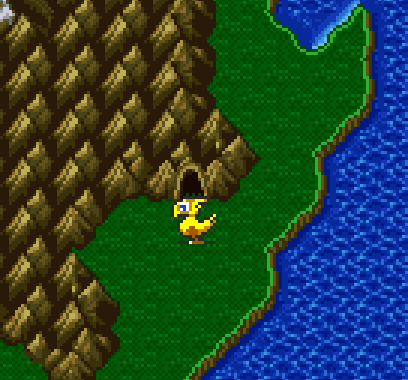
\includegraphics[scale=0.392]{../Graphics/Misc/18. Chocobo Discount.png}
\end{misc}

\switchcolumn*
\begin{enumerate}[resume]
    \item Head to the Pyramid of Moore
    \item Avoid this tile at the Elder Tree
\end{enumerate}

\switchcolumn
\begin{misc}{Elder Tree Cutscene Tile}
    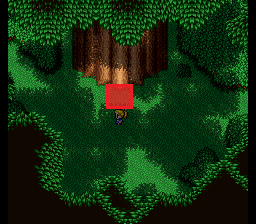
\includegraphics[scale=0.626]{../Graphics/Misc/19. Elder Tree Cutscene Tile.png}
\end{misc}

\switchcolumn
\begin{menu}{Before Entering the Pyramid}
    \varwb
    \begin{jobMenu}
        \cara Samurai \textbf{(\pointLeft)(\pointDown)} \ability{\dash} \optimize
        \faris Ninja \textbf{(\pointLeft)(\pointDown)(\pointLeft) \ability{!\gilToss}}
    \end{jobMenu}
    \begin{itemMenu}
        \hiPotionMenu \ally{People missing 100+ HP}
    \end{itemMenu}
    \varwe
\end{menu}

\end{paracol}